\documentclass[11pt]{article}
\usepackage[english]{babel}\usepackage[a4paper, margin=1.5cm]{geometry}
\usepackage{hyperref}
\usepackage[authoryear]{natbib}
\usepackage{graphicx}
\usepackage{setspace} % Set line spacing
\usepackage{float}
\usepackage{array}
\usepackage{caption}
\usepackage{booktabs}



\setstretch{1} % Single line spacing

\title{DevOps, Software Evolution and Software Maintenance}
\author{mkrh, mahf, jkau, lakj, ezpa \\
\url{https://github.com/group-o-minitwit-2024/MiniTwit}\\
\url{http://group0minitwit.lol}\\
\url{http://group0minitwit.lol/api}
}

\date{23 May 2024}

\begin{document}

\maketitle

\section{System's Perspective}
\subsection{Technology Stack}
Our technology stack, as seen in figure \ref{fig:dev-stack}, consists of Express.js and Node.js for both the front-end and back-end, utilizing JavaScript, Mocha, and WebdriverIO for end-to-end testing. Our database is managed by a PostgreSQL server and queried from the frontend with the ORM package Sequelize. It is hosted on a database cluster provided by Digital Ocean. The application itself is deployed on a Digital Ocean droplet. For monitoring and observability, we employ Prometheus for collecting metrics, and visualize the metrics using Grafana. Containerization and orchestration are handled by Docker and Docker Swarm, respectively. Continuous Integration and Continuous Deployment (CI/CD) pipelines are automated through GitHub Actions. Logging of MiniTwit is managed using the EFK (Elasticsearch, Filebeat, Kibana) stack.

\begin{figure}[!h]
    \centering
    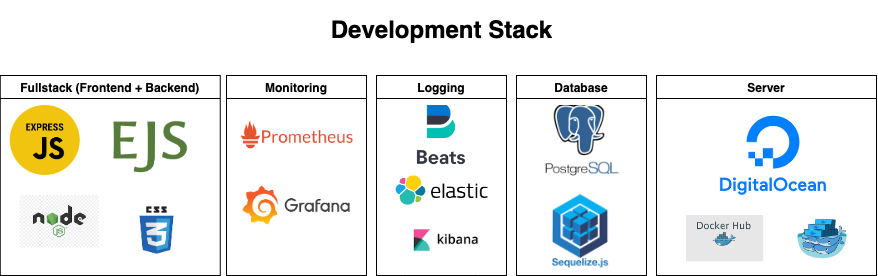
\includegraphics[width=\textwidth]{images/techstack.png}
    \caption{Overview of development stack, with each element grouped by use case.}
    \label{fig:dev-stack}
\end{figure}

\subsubsection{Arguments for Choice of Technology Stack}
\textbf{Express.js}, built on Node.js, is renowned for its non-blocking, event-driven architecture, which enhances performance and scalability and is well build and modern maintained programming language. By leveraging Express.js, we unify our technology stack under JavaScript for both front-end and back-end development which is neat for a simple webpage. Express.js integrates well with a wide array of modern development tools and services due to the extensive eco system of npm packages. Everything from PostgreSQL, Sequelize, WebdriverIO to small packages like express-flash (that made the refactor more simple).

Furthermore, JavaScript is the most used programming language in the world \citep{javascript_good}. When working in an interdisciplinary team with different backgrounds and skill sets, one should choose a language that all members can actively contribute to, even if they have no prior experience with the specific language. JavaScript fulfills this criteria, with it being a widely known, high level programming language, and extensively documented. This allowed every member to contribute to the development of the app, whereas a lower level language with a higher barrier to entry would discourage collaboration. 


\subsubsection{Arguments for choice of Virtualization Techniques and Deployment Targets}
Docker is a great choice for making environments portable across different systems and machines. It encapsulates the dependencies needed for development and the use of Docker Hub allows to centralize the repository for the docker images. Furthermore, we implement Docker Swarm so that we can scale our service horizontally across multiple hosts. When coupled with Terraform, it enables us to easily scale the amount of droplets for the swarm based on demand. Docker was voted \#1 Most-used developer tool by Stack-Overflow 2023 Developer Survey \citep{docker_no1} and therefore familiarising ourselves with it can improve our CV and work opportunities.
The choice of Digital Ocean as a cloud provider was mainly based on recommendations and cost. Cloud providers can be very expensive and Digital Ocean provided us with a 200 USD free spending cap since we are students.

\subsubsection{Current state of system}
We use Sonarcloud as a static code analysis tool, which has generated a security report using Bitegarden's report for Sonarcloud. The report can be accessed at: \url{https://group-o-minitwit-2024.github.io/}. 



\section{Process' Perspective}
The following diagram describes the Process Development Landscape:
\begin{figure}[!h]
    \centering
    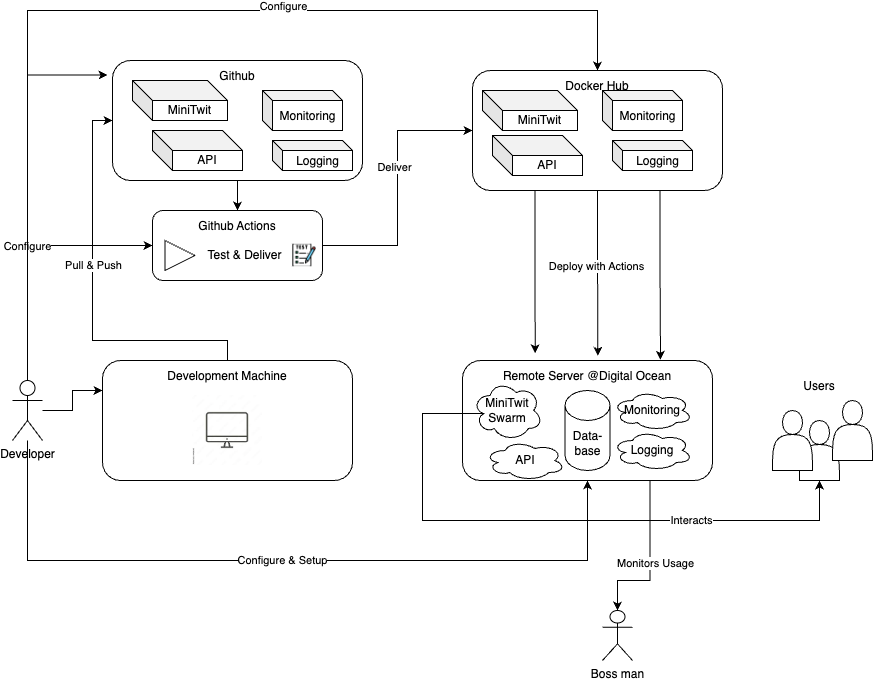
\includegraphics[width=\textwidth]{images/process.png}
    \caption{Process' Landscape}
    \label{fig:process-overview}
\end{figure}

The process can be describe as follows: A developer works on his local machine. From there he can push and pull to the Github repository. The developer can work with Docker images or completely locally with npm start. The Github repository is setup with Github Actions that automates tasks such as linting, testing, building, and pushing changes to Docker Hub. Furthermore, Github Actions has automated workflow for pulling Docker images from Docker Hub and deploying them to our cloud provider Digital Ocean. The developer has scripts that automates the setup of infrastructure on Digital Ocean using Terraform. From this step the application is live and configured. Users interact with the application by pinging the Minitwit webpage hosted on Digital Ocean. 

\subsection{Implementing CI/CD with GitHub Actions}

We use the following workflows in GitHub Actions:
\begin{itemize}
    \item \textbf{ESlint}: Linting tool for Javascript
    \item \textbf{Hadolint}: Linting tool for Dockerfiles
    \item \textbf{Sonarcloud} Detects bugs, vulnerabilities, and code smells
    \item \textbf{Endpoint Tests}: Automated tests to test API endpoints.
    \item \textbf{Deploy}: Automated pulling and deployment to production server
    \item \textbf{Report}: Automated compile and build of LaTex report to PDF. PDF is uploaded to main branch.
    \item \textbf{Weekly Release}: Automated Weekly release of the main branch.
\end{itemize}

For our CI/CD pipeline we use GitHub Actions. A study shows that GitHub Actions has become the most popular CI service, surpassing older, popular options like Jenkins and Travis CI \citep{github_actions_good}. The authors of the paper provide several reasons for this shift. First and foremost is the seamless integration with GitHub. GitHub Actions benefits from its native integration with GitHub repositories. This close integration simplifies setup, maintenance, and overall workflow, making it a superior choice compared to other CI services like Travis CI or Jenkins, which might require additional configuration for GitHub projects. This seamless integration ensures that changes made in the repository are immediately reflected in the CI/CD process. 
Secondly, GitHub Actions offers predefined workflows and a wide array of reusable actions, significantly simplifying the setup of CI/CD pipelines. This feature allows us to quickly implement robust pipelines without needing to build everything from scratch. This approach not only speeds up the development process but also reduces the potential for errors, as these actions are maintained by the community and are regularly updated.
Thirdly, cost-effectiveness plays a major role as well. GitHub Actions offers a free tier, which gives an advantage for open-source projects and smaller teams like ours. \\
The paper argues that these three points are a big contributor to the rise of GitHub Actions in the CI\/CD space. Moreover, with more users adopting GitHub Actions, there are more forum posts, blog posts, guides, and tutorials available, increasing our odds of finding solutions to problems we encounter or detailed guides to specific workflows we need to implement. 



\subsection{How do you monitor your systems and what precisely do you monitor?}

For system monitoring, we use \textit{Prometheus} and \textit{Grafana}. These services are separated from the rest of MiniTwit into their own repository\footnote{\url{https://github.com/group-o-minitwit-2024/MiniTwit-monitoring}}. We use Prometheus for collecting metrics from both \textit{MiniTwit} and \textit{MiniTwit-api}. To this end, both applications expose a \texttt{/metrics} endpoint that exposes metrics for Prometheus to scrape. Prometheus regularly scrapes all of MiniTwit for these metrics, as defined in the \href{https://github.com/group-o-minitwit-2024/MiniTwit-monitoring/blob/main/prometheus/prometheus.yml}{\texttt{prometheus.yml}} file. It is configured for both collecting metrics from the production system as well as a local instance. 

Grafana is used to aggregate and visualize data collected by Prometheus. It integrates natively with Prometheus as a datasource, which is automatically configured through Grafana's \href{https://github.com/group-o-minitwit-2024/MiniTwit-monitoring/blob/main/grafana/provisioning/datasources/datasources.yaml}{\texttt{datasources.yml}} configuration file. A dashboard is also automatically setup with some of the metrics Prometheus collects. 

With this Prometheus and Grafana stack, we collect real-time information about MiniTwit's current traffic and state, as seen in figure \ref{fig:grafana}. Specifically, we currently monitor CPU usage, the rate of traffic and the response time distribution, all of which are shown for both the app and the api. These metrics are collected and monitored, as they give an indication of the overall system state, if it is overloaded, and if it is experiencing slow response times; all of which are crucial to control in a production environment. The biggest thing missing from the current dashboard is insights into the state of the database. Since the database is arguably the most influential aspect of the tech stack, we should monitor its status, load, performance etc. Additionally, the current setup only monitors a single instance of MiniTwit. However, in newer iterations of the app, we run the app with Docker Swarm with replication, which would be both be beneficial to monitor, and breaks backwards compatibility. 

\begin{figure}[h]
    \centering
    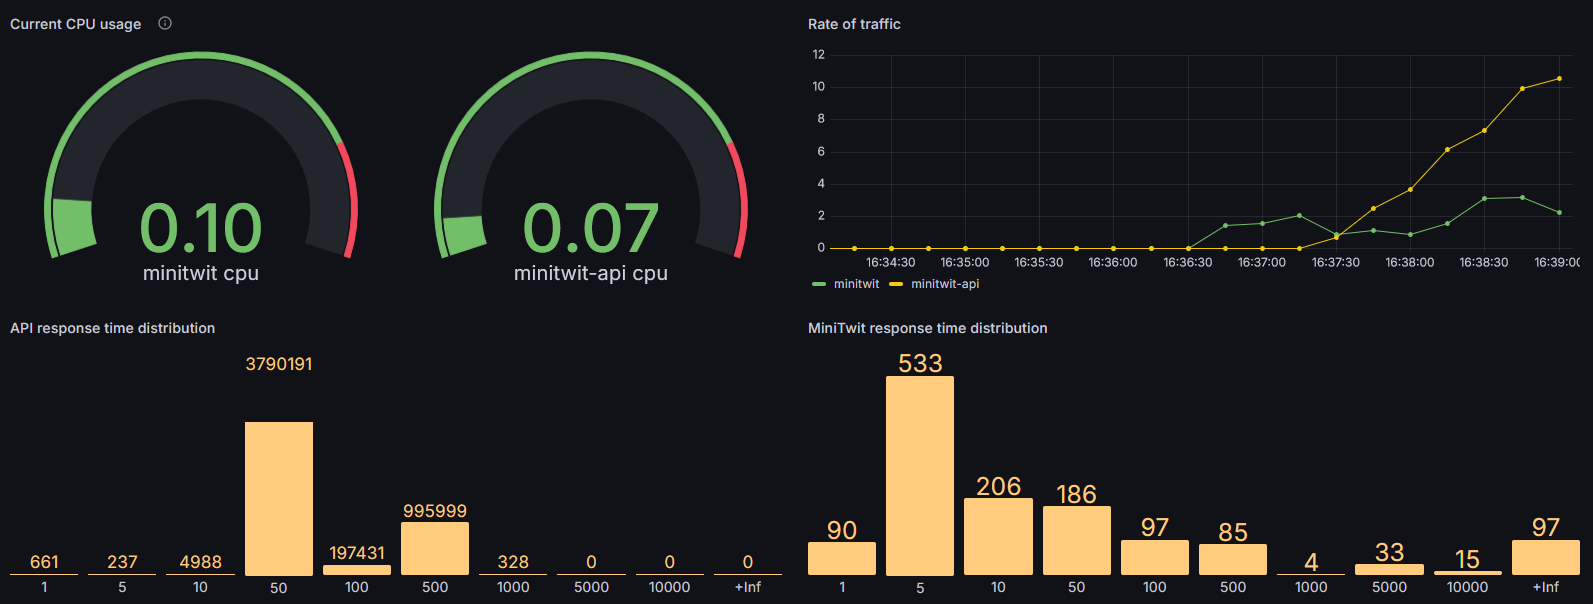
\includegraphics[width=0.75\linewidth]{images/grafana.png}
    \caption{Screenshot of the Grafana dashboard showcasing the current state of the production MiniTwit system.}
    \label{fig:grafana}
\end{figure}



\subsection{What do you log in your systems and how do you aggregate logs?}
With our EFK stack we plan to log every single interaction a user might have with the website, as well as all the logs provided by Docker. The sequelize.js file logs each user interaction to the console. Provided we had the time, Winston\footnote{\url{https://github.com/winstonjs/winston}} would have been our preferred logging implementation, as it allows for additional logging capabilities. There are mainly two improvements for using Winston over Sequelize: Winston has 7 logging levels, ranging from 0 to 6 and the severity of all levels is assumed to be numerically ascending from most important to least important. This conforms to the severity ordering specified by RFC5424 \citep{rfc5424}. Secondly, Winston allows for the logs to be saved to a specified file, instead of only writing to the console. 
In our \texttt{filebeat.yml} file, we specify a process called \textit{add\_docker\_metadata}, which annotates each event with relevant metadata from Docker containers\footnote{\url{https://www.elastic.co/guide/en/beats/filebeat/current/add-docker-metadata.html}}. This ensures that all logs are enriched with context about their source.\\
Logs collected by Filebeat are sent to Elasticsearch, where they are indexed and stored. Using Kibana, we create two index patterns: one for logs from the website and another for logs from Docker. This setup allows us to efficiently search, analyze, and visualize logs from different sources in a centralized location. By aggregating logs in this manner, we can monitor system performance, troubleshoot issues, and gain insights into user behavior. An example of a few logs Docker are shown below:

\begin{figure}[h]
    \centering
    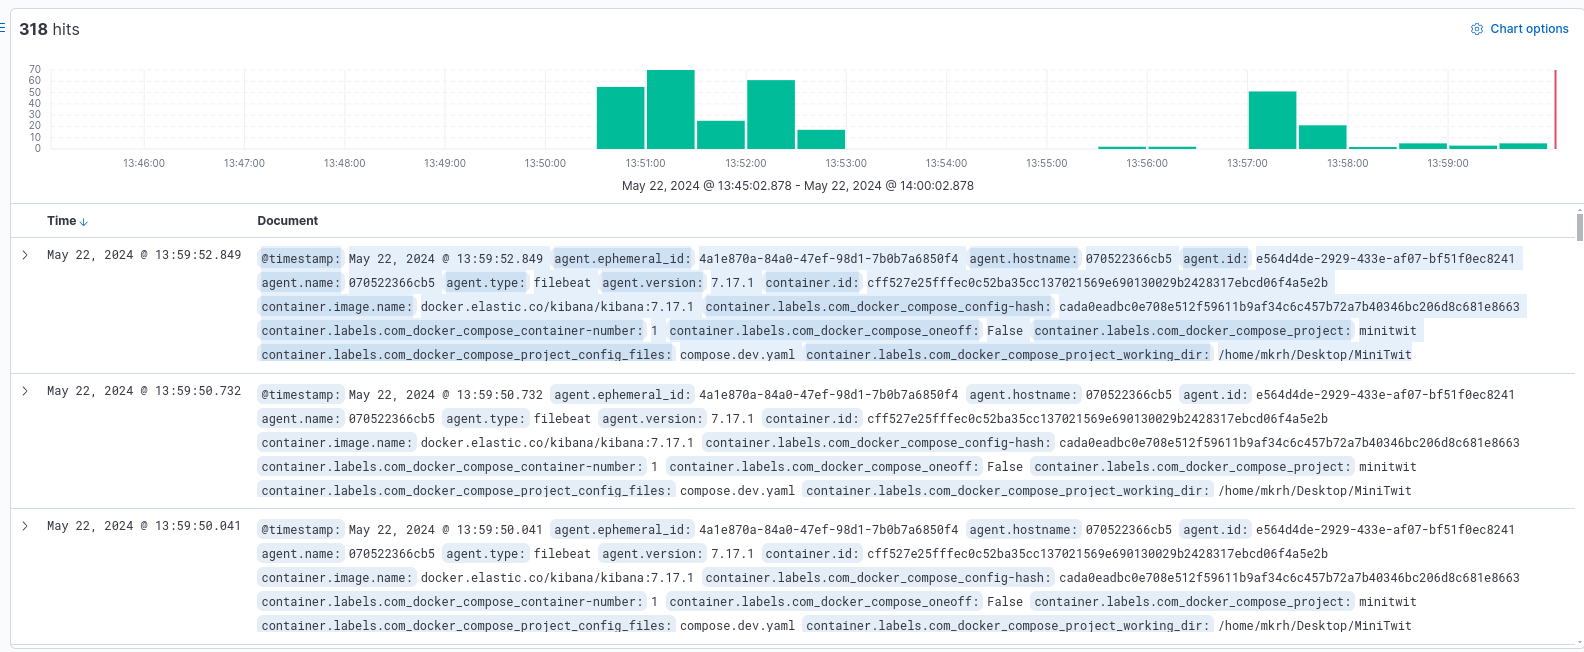
\includegraphics[width=0.85\linewidth]{images/efk_docker_logs.png}
    \caption{The screenshot displays the last three Docker log entries in Kibana, including metadata like timestamp, agent information, container ID, image name, and Docker Compose labels}
\end{figure}
Unfortunately, due to droplet size constraints, we were not able to download the images needed for the EFK stack. A fix for this is to provision a bigger droplet. However, we did not have the credits for this. Therefore, the logging setup is not a part of the main branch, but lives on its own branch at: \url{https://github.com/group-o-minitwit-2024/MiniTwit/tree/logging_branch}

\subsection{Applied strategy for scaling and upgrades}
Depending on the phase of the project, we applied different strategies for improving the system. In the beginning, we scaled our system vertically, upgrading the database and the droplet node in resources when we experienced limitations. Due to the service running on a single node, we would have downtime whenever we pulled changes and re-deployed. However, now, we are running on a Docker Swarm cluster with services replicated across multiple nodes. This allows us to use a rolling update strategy, where each service is updated one node at a time, resulting in $100\%$ uptime. Additionally, this also allows us to scale horizontally, where the load is shared between replicas instead of all traffic being directed at a single machine. 


\subsection{Role of AI in the development process}
During the development of the system, various AI technologies have empowered the development team in the process of conducting requirements elicitation for the application in order to implement the presented solutions. We have utilized OpenAI’s ChatGPT and Google's Gemini models to analyze and decompose the different elements that constituted the target implementations during the development cycle. The use of these technologies has provided rapid insights and guidance, accelerating the learning curve in the understanding process of implementations.


\subsection{Risk assessment}
\subsubsection{Risk Identification and Analysis}
 We present table \ref{tab:risk-assessment} as a summary of risk assessments. We prioritize the risks based on their combined likelihood and impact. We also include the mitigation strategies in the table to make it easier to get an overview. The table is in ranked order, from highest priority to lowest. The highest priority risks are those with high likelihood and high impact, such as SQL Injection Attacks, Data Breaches, and Software Vulnerability Exploits. We base our findings on Sonarcloud's produced report on our application as well as researched security threats and mitigation strategies.
 
We use these classifications: 
\begin{itemize}
    \item Likelihood: {Certain, Likely, Possible, Unlikely, Rare}
    \item Impact: {Insignificant, Negligible, Marginal, Critical, Catastrophic}
\end{itemize}

\subsubsection{Brief Risk Identification}
The primary risks  we have identified for our web application include SQL injection attacks, data breaches, DDoS attacks, unauthorized access, data loss, and software vulnerability exploits. According to the OWASP Top Ten, SQL injection and data breaches remain critical security risks due to their prevalence and potential impact on sensitive information \citep{owasp_top_ten}. Sonarcloud identified the following security hotspots for our application:

\begin{enumerate}
    \item Hard-coded credentials are security-sensitive (js) 
    \item Hard-coded credentials are security-sensitive (py)
    \item Recursively copying context directories is security-sensitive (docker)
    \item Allowing shell scripts execution during package installation is security-sensitive (docker)
    \item Running containers as a privileged user is security-sensitive (docker)
    \item Disclosing fingerprints from web application technologies is security-sensitive (js)
\end{enumerate}

To mitigate these risks, we have several strategies (see table \ref{tab:risk-assessment}). We use ORMs like Sequelize to help prevent SQL injection attacks, as recommended by OWASP \citep{owasp_sql_prevention}. For future development, we should encrypt sensitive data, salt passwords, and enforce HTTPS ensures secure data transmission, as per NIST guidelines \citep{nist_tls}. 


\begin{table}[H]
    \centering
    \caption{Risk Assessment}
    \begin{tabular}{|p{3cm}|p{2cm}|p{2cm}|p{7cm}|}
        \hline
        \textbf{Risk} & \textbf{Likelihood} & \textbf{Impact} & \textbf{Mitigation Strategy} \\Ideally we could implement multi-factor
        \hline
        SQL Injection Attack & Likely & catastrophic & We use the ORM Sequelize to avoid raw queries. We should regularly update dependencies. With our monitoring we should try to review the database logs and performance metrics for any suspicious access patterns and unusual spikes. \\
        \hline
        Data Breach & Possible & Catastrophic & We hash sensitive data like passwords and are working on implementing HTTPS (as per writing). We also follow REST API principles. However Sonarcloud points out an issue with HTTP request redirections being open, which we should remedy. Generally we should strive to enforce strong authentication and authorization practices. Looking ahead implementing Automating Pen Testing
        would be a good strategy. We should also consider implementing security monitoring tools to detect and respond to breaches in close to real-time. \\
        \hline
        DDoS Attack & Possible & Critical &  We scale using Docker Swarm to try to distribute the system load, however this is by no  means a fix all. Implementing some kind of  DDoS protection, like rate limiting should be considered. Again here, monitoring for suspicous patterns, and the like is something we should include in our strategy. We can for instance set up alerts for sudden increases in traffic. \\
        \hline
        Data Loss & Unlikely & Catastrophic & There is functionality for backups with the PostgreSQL database, however automatic backups was decided against due to cost. Looking ahead we could  implement disaster recovery plans. \\
        \hline
        Software Vulnerability Exploits & Likely & Critical & First of all we should make sure that software components are regularly updated. Dedicated vulnerability / security scans as CI GitHub Actions like Metasploit or snyk  should also be considered as something to implement. Although currently Sonarcloud do uncover some vulnerabilities.  \\
        \hline
        Resource Exhaustion (CPU/Memory) & Rare & Critical & We monitor system performance with Prometheus. We also scale resources using Docker Swarm, and use load balancing which should help optimize the application for performance. \\
        \hline
        Unauthorized Access & Possible & Marginal & We currently have a simple password policy, but should strive to improve it in future iterations. Ideally we could implement multi-factor authentication. Monitoring is also relevant here to detect unauthorized access.  \\
        \hline
    \end{tabular}
    \label{tab:risk-assessment}
\end{table}

\section{Lessons Learned Perspective}
The biggest lessons learned relate to the overall structuring and development of a larger collaborative project. While we attained significant hands-on experience with new tools and technologies, we found more value in learning to work together in a team with widely varied skill sets and backgrounds. When someone initially developed features early in the project, we would spend great time knowledge sharing and ensuring everyone understood, what was going on. However, as we got further into the project, less knowledge was shared, while no documentation was written, leading to a decrease in productivity, as it became an increasingly daunting task to develop on the evergrowing complex system. This issue influenced the teams productivity both in terms of maintenance and evolution, since it was hard to work on elements without any knowledge. This is reflected in many of our GitHub Issues being left open for months at a time, preventing an agile workflow. One example of this is seen in the issue \href{https://github.com/group-o-minitwit-2024/MiniTwit/issues/37}{\textit{"Race condition with regards to database initialization and app execution in compose \#37"}}. This maintenance task was left open for approximately 2 months, despite its relative simplicity. The biggest factor as to why this was not solved sooner is the lack of knowledge sharing, which turned a simple maintenance task into a whole self study on the infrastructure and networking of the app. This is just one example, but has been a problem all throughout the project. \\

Another lesson learned is that we should prioritize the integration of new features. When working, we had a tendency to try to perfect every little detail of an implementation before merging, leading to long development times, and minimal feedback. This had the consequence of work being invisible, and when something was finally done, there would be a huge batch of code that needs merging with the master branch and to be deployed. This is contradictory to the principle of flow \citep{devops_handbook}, where work should be visible and often integrated. It also meant that there was no feedback flow, leading to stagnating development. One example of this is with our integration of \textit{Docker Swarm} and \textit{Terraform}. Both of these individually are huge steps which have major ramifications for the existing code and infrastructure. However, both was developed on one branch and merged in the same pull request (see pull request \href{https://github.com/group-o-minitwit-2024/MiniTwit/pull/64}{\textit{"Docker Swarm and Infrastructure as code \#64"}}), leading to a longer than needed development time, a huge bulk of code, and a lot of minor details that needed tuning in production. In retrospect, it would have been better to either do Docker Swarm first, or do both of them in parallel but separated with smaller incremental developments. \\


Lastly, we learned that we should be less scared of failure. As an extension of both of the previous points, many tasks were left untouched for much longer than they should due to the fear of breaking existing code or infrastructure. This is particularly true for aspects pertaining to the production database. For instance, the issue \href{https://github.com/group-o-minitwit-2024/MiniTwit/issues/57}{\textit{"Response time of MiniTwit is getting immensely slow \#57"}} was open for a month, despite being solved a week after the issue was created. Fear of messing up the system played a major role in this and delayed maintenance tasks, even though the fix was simple.


% \begin{itemize}
%     \item A lot of new tech tools
%     \item Sharpened proficiency of already known tools
%     \item Working in a collaborative environment - with different backgrounds
%     \item Formal procedures for planning and distributing work
%     \item Working in a larger team - how do we share knowledge and coordinate work with a lot of conflicting schedules
%     \item Maintenance is difficult, boring, hard (particularly on production infrastructure). 
% \end{itemize}


% Describe the biggest issues, how you solved them, and which are major lessons learned with regards to: evolution and refactoring, operation, and maintence of your ITU-MiniTwit systems. Link back to respective commit messages, issues, tickets, etc. to illustrate these.
% Also reflect and describe what was the ”DevOps” style of your work. For example, what did you do
% differently to previous development projects and how did it work?\\
% \textit{Taken from slides/prep document: }The following general steps will guide you through a security assessment. Consider using them as steps in a report. The report will become a section in your final project report.




\newpage
\bibliographystyle{chicago} 
\bibliography{references}

\newpage

% \newpage

\subsection{What to include in the report?}

\subsubsection{System's Perspective}

A description and illustration of the:

\begin{itemize}
    \item Design and architecture of your \textit{ITU-MiniTwit} systems
    \item All dependencies of your \textit{ITU-MiniTwit} systems on all levels of abstraction and development stages. That is, list and briefly describe all technologies and tools you applied and depend on.
    \item Important interactions of subsystems
    \begin{itemize}
        \item For example, via an illustrative UML Sequence diagram that shows the flow of information through your system from user request in the browser, over all subsystems, hitting the database, and a response that is returned to the user.
        \item Similarly, another illustrative sequence diagram that shows how requests from the simulator traverse your system.
    \end{itemize}
    \item Describe the current state of your systems, for example using results of static analysis and quality assessments.
\end{itemize}
MSc should argue for the choice of technologies and decisions for at least all cases for which we asked you to do so in the tasks at the end of each session.

\subsubsection{Process' perspective}

This perspective should clarify how code or other artifacts come from idea into the running system and everything that happens on the way.

In particular, the following descriptions should be included:

\begin{itemize}
    \item A complete description of stages and tools included in the CI/CD chains, including deployment and release of your systems.
    \item How do you monitor your systems and what precisely do you monitor?
    \item What do you log in your systems and how do you aggregate logs?
    \item Brief results of the security assessment and brief description of how did you harden the security of your system based on the analysis
    \item Applied strategy for scaling and upgrades
\end{itemize}
In case you have used AI-assistants during your project briefly explain which system(s) you used during the project and reflect how it supported/hindered your process.

\subsubsection{Lessons Learned Perspective}

Describe the biggest issues, how you solved them, and which are major lessons learned with regards to:

\begin{itemize}
    \item evolution and refactoring
    \item operation, and
    \item maintenance
\end{itemize}
of your \textit{ITU-MiniTwit} systems. Link back to respective commit messages, issues, tickets, etc. to illustrate these.

Also reflect and describe what was the "DevOps" style of your work. For example, what did you do differently to previous development projects and how did it work?


 Taken from slides/prep document:

The following general steps will guide you through a security assessment. Consider using them as steps in a report. The report will become a section in your final project report.

\subsubsection{A. Risk Identification}

\begin{enumerate}
    \item Identify assets (e.g. web application)
    \item Identify threat sources (e.g. SQL injection)
    \item Construct risk scenarios (e.g. Attacker performs SQL injection on web application to download sensitive user data)
\end{enumerate}

\subsubsection{B. Risk Analysis}

\begin{enumerate}
    \item Determine likelihood
    \item Determine impact
    \item Use a Risk Matrix to prioritize risk of scenarios
    \item Discuss what are you going to do about each of the scenarios
\end{enumerate}



\section{Appendix}
\begin{figure}[!h]
    \centering
    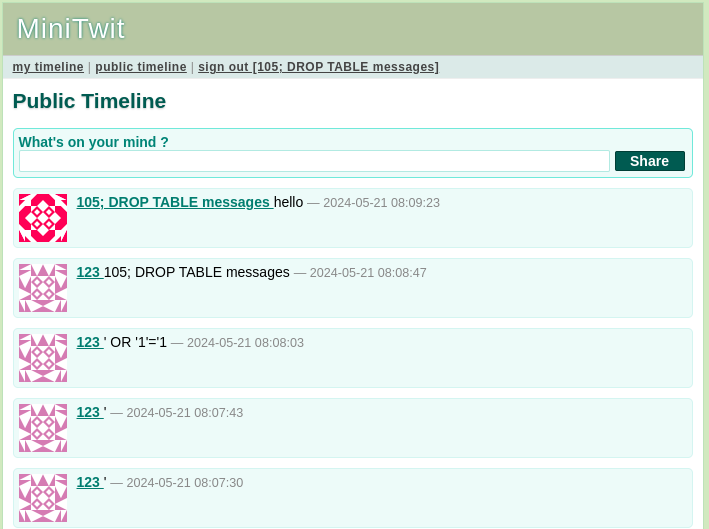
\includegraphics[width=0.8\textwidth]{images/sql_injections.png}
    \caption{Example of user input being sanitized and the system is not open to these kind of injections}
    \label{fig:sqlinjections}
\end{figure}



\end{document}